\chapter{Reproducible NMR data set}

\begin{center}
  \textit{Our responsibility is to do what we can, \\* learn what we can, 
    improve the solutions, and pass them on.}

 - Richard Feynman
\end{center}

% TODO make sure to point out that there's multiple ways to do this
% there's different NMR-domain approaches
% but there's also both the git-based and NMR-STAR-based approaches

In order to prove the validity of the approach described in the previous
chapter, it was applied to typical NMR data in order to solve a protein
structure.  The process was carried out in full, and sufficient data was
captured during the process in order to render it reproducible.


\section{Methods and Materials}

Time-domain data of Samp3, a Ubiquitin-like protein, were kindly provided by 
Dr. Mark Maciejewski.  The data were processed to frequency-domain spectra
using NMRPipe, and then analyzed first in CCPN Analysis \cite{ccpn} and later 
in Sparky \cite{sparky}.  A preliminary analysis process used CCPN Analysis,
along with git and several Python utilities to create and manage the 
reproducible history.  The final analysis used Sparky, the model and approach
described in the previous chapter, the extension described in the following
chapter, and the extensions to the NMR-STAR data dictionary.  
Cyana was used to assign NOEs,
disambiguate stereospecific assignments, and calculate structure bundles.
% TODO more detail?  pictures?


\section{The analysis process}
Starting from time-domain data sets, I carried out the standard data analysis
process using a subset of the CCPN data model \cite{ccpn}, 
with the additional property that the process itself was captured as
a series of annotated snapshots, and extraneous results were recorded as well.
The full data set including complete annotated snapshot history may be found at 
\url{https://github.com/mattfenwick/samp3}
(a previous version using the CCPN Analysis program may additionally be found
at \url{https://github.com/mattfenwick/PeakPicker/tree/ab3}).
A summary of the process is described here.

\subsection*{Initial peak picking and GSS construction}
First, the NHSQC and HNCO spectra were peak picked using an automated 
peak picker; see Table \ref{samp3_spectra} for a complete list of spectra
used.  Then GSSs were built based on NHSQC peaks and matching HNCO peaks
according to the H and N dimensions.  Peaks either in the NHSQC or HNCO
which did not match peaks in the other spectra were verified manually, and
many were labeled as extraneous and not included in GSSs.

Several sidechain spin systems, including Asparagine, Glutamine, Tryptophan,
and Arginine, were identified based on either peaks with matching N and C
chemical shifts but different H shifts, spectral position, or peak intensity
combined with splitting.  An example of an Asparagine sidechain is shown in
Figure \ref{asn_sidechain}.  Several factors allow these peaks to be grouped
into a single GSS, and that GSS to be typed as an Asparagine:
\begin{itemize}
  \item two peaks in the NHSQC with matching N frequencies, but different H
    frequencies, in the top right of the spectrum.  These are caused by the
    two non-equivalent protons on the sidechain N.
  \item two additional, less intense peaks in the NHSQC matching the two
    H frequencies but at a lower PPM in the N dimension.  These are caused by
    a small fraction of the sample which has one D and one H.
  \item two peaks in the HNCACB matching each of the D/H peaks in the NHSQC,
    and matching each other as well.  These are caused by the CB and CA; 
    however, the signs of the peaks are swapped from what they should be for
    a backbone GSS, since the CB is now closer to the H-N group than the CA.
  \item characteristic chemical shifts which match a CB/CA of Asparagine, 
    and do not match a CG/CB of Glutamine.
\end{itemize}

\subsection*{GSS and resonance typing}
Analysis continued with peak picking of the HNCACB and C(CO)NH-Tocsy spectra.
The inclusion of the H and N dimensions allowed these peaks to be added into
GSSs based on the matching of these two chemical shift values to the
root peaks of existing GSSs.  There was some H/N overlap which complicated the
task of unambiguous peak-GSS assignment, but it was mostly resolved through
the extra Carbon dimensions, which allowed peaks to be identified separately
and with more precise chemical shift values.

The overlap between the two spectra -- peaks of sidechain i-1 Carbons, relative
to a backbone amide group, appeared in both spectra, while only the i peaks
appeared in the HNCACB -- allowed for assignment of resonance type of HNCACB
peaks and some C(CO)NH-Tocsy peaks.  Additionally, for GSSs with more than two
i-1 Carbon atoms, the C(CO)NH-Tocsy resonance typings were simplified by the
removal of CA and CB assignment possibilities due to overlap with the HNCACB.

The Carbon chemical shifts provided sufficient information for GSS typing
in many cases.  The number of peaks in C(CO)NH-Tocsy strips also provided 
information about the typing of the previous GSS, the use of which is described
in the following section.

\subsection*{Sequential and residue-specific GSS assignment}
GSSs were built into sequential chains based on overlap of CA(i) and CB(i) 
peaks of one GSS with CA(i-1) and CB(i-1) peaks of another.  It was critical
that the overlap be unambiguous; ambiguous overlaps were deferred until later
when additional information would provide disambiguation.
Simultaneously, chains were assigned to residue sequences based on GSS typing
and chain order matching the residue typing and chain order.  GSS chains
were often anchored on a Glycine, Serine, Threonine, or Alanine residue due
to their unique Carbon chemical shifts.

The whole process was heavily interdependent for several reasons.  First, by
assigning a GSS chain to specific residues, the typing for the GSSs both
immediately preceding, and immediately following the first and last GSSs,
respectively, of the chain were implied; this narrowed the search for further
GSSs to those either with the appropriate typing, or an unassigned typing but
with chemical shifts that matched the average BMRB statistics sufficiently 
well.  It was also necessary that these GSSs were not already assigned as 
part of a GSS chain because ambiguous assignments were disqualified.
Second, assigning a GSS chain to residues reduced the number of unassigned
residues, and therefore the number of possibilities for other unassigned chains
as well.  It was several times the case that assigning a chain led immediately
to the assignment of another chain by the process of elimination.  Third,
assigning GSSs sequentially narrowed the number of places in the sequence that
could potentially accomodate the chain, both because of the chain-ending
constraints imposed by Proline residues as well as the necessity of matching
all GSS typing to residue typing.

\subsection*{Sidechain: GSS augmentation and resonance typing}
The C(CO)NH-Tocsy provided information on the chemical shifts of aliphatic
sidechain carbons, as covered in the previous section.  The HBHA(CO)NH, 
HC(CO)NH-Tocsy, and HCCH-Tocsy provided the chemical shifts of aliphatic
protons, as well as additional corroborating information of aliphatic carbons.

First, these spectra were peak picked, as before, by an automated peak picker.
The results were then corrected in a coarse validation step, before assembling
the peaks into GSSs based on matching chemical shifts.  For the HC(CO)NH-Tocsy
and HBHA(CO)NH spectra, this was based on matching of backbone H and N
resonances and was unambiguous for the most part.  The HCCH-Tocsy, lacking these
resonaces, was based on matching to sidechain H and C resonances, and was
slightly more difficult to interpret due to ambiguities.  
Average BMRB statistics as well as peak patterns based on prochiral methylene
groups were sufficient for resonance typing.
% TODO show some HCCH-Tocsy strips

\subsection*{Aromatic assignment}
The two final through-bond experiments, the hbCBcgcdHD and hbCBcgcdceHE, were
used to find the HD and HE resonances of aromatic sidechains and place them
into the correct GSS.  The spectra were again peak picked with an automated
peak picker, and then assigned by matching the C dimension with the previously
analyzed CB chemical shifts: the GSS with a matching CB(i) resonance was the
appropriate one.

\subsection*{NOE assignment and structure calculation}
The four NOESY spectra were peak picked with an automated peak picker.  
Talos+ \cite{talos+} was run on the chemical shift assignments of the H, HA,
CA, CB, CO, and N nuclei in order to generate Phi and Psi torsion angle 
constraints for backbone conformation.
The Talos+ results can be seen in Figure \ref{talos+_results}.

Cyana was then run by providing it the NOESY peak lists, chemical shift
assignments, torsion angle constraints, and Samp3 sequence.  The script
used for running Cyana is shown here:
\begin{verbatim}
# NOESY peak lists in XEASY format
peaks       := aromatic_gnoesy_chsqc.pks,aromatic_noesy.pks,
               D2O_noesy_chsqc.pks,noesy_nhsqc.pks
# names of chemical shift lists
prot        := shifts.txt                
# additional (non-NOE) restraints
restraints  := aco.aco                   
# shift tolerances: H, H', C/N', C/N
tolerance   := 0.04, 0.03, 0.45          
# number of initial, final structures
structures  := 100,20                    
# number of torsion angle dynamics steps
steps       := 10000                    
# random number generator seed
randomseed  := 434726                    

nproc=8

noeassign peaks=$peaks prot=$prot autoaco
\end{verbatim}
After running Cyana once, the output indicated issues with stereospecificity
of certain assignments (methylene protons, as well as Leucine and Valine
CG groups).  These assignments were corrected according to Cyana's feedback,
and Cyana re-run with the corrected stereospecific assignments.
The final structure is shown in Figure \ref{structure} as seen in jmol.


% \section{NMR-STAR data set} TODO
% TODO get the data set
% what should I talk about here?  the various approaches and deductions used?
% queries performed on the data, that show certain things?
% the order in which I did things?


\section{Archiving reproducible data sets}
A major portion of the value derived from collecting reproducible data sets
is disseminating them so that others may obtain and use or inspect the data
in some way.  The standard means for sharing NMR-derived data is the BMRB
\cite{bmrb}, which uses the NMR-STAR file format.  In order to enable archival
of reproducible data sets, we have collaborated with the BMRB to extend the
NMR-STAR data dictionary, so that reproducible data sets may be collected and
deposited in the NMR-STAR format.

The NMR-STAR data dictionary, which may be found at 
\url{http://www.bmrb.wisc.edu/dictionary/}, catalogs the names, structure,
intended use, and definitions of the data types handled by the BMRB.


\section{Assessing the difficulties encountered}
NMR data analysis must deal with the inherent issues of false positives, false 
negatives, ambiguity, and extraneous data.
Presented here is a quantification of these problems which were encountered
during several phases of analysis.

\subsection*{NHSQC peak pick}
The NHSQC peak pick is a critical component of analysis because it is used
to find the GSS roots, off of which may be based the restricted peak picks of
the three-dimensional triple-resonance experiments.
Table \ref{nhsqc_peakpick} gives an overview of the results.
The precision of the peak pick was 99 / 105 = 94.3\%{}; the 6 false positives 
were likely caused by sinc wiggles from an extremely intense peak, as they
matched the 1H chemical shift of a signal peak, and there were not matching
signals found in the three-dimensional spectra.
The recall was 99 / 118 = 83.9\%{}, and the 
F1-score was 2 * precision * recall / (precision + recall) = 88.8\%{}.
See Figure \ref{false_negative} for an example of a false negative.

\subsection*{Completeness of observed NMR signals in NHSQC}
Whether a signal is observable in NMR experiments is not always predictable
directly from the primary sequence:  it may depend on the structure and
dynamics of the molecule.  Table \ref{nhsqc_signals} presents the numbers
of expected signals based solely of off the primary sequence, and of found 
signals, based off of the chemical shift assignments.  Note that an 
extraneous GSS was found that could not be fit into the sequential assignments
(See Figure \ref{extraneous_gss}).

\subsection*{Overlap in the NHSQC}
Overlap presents difficulties during both sequential and NOESY assignment
because individual signals are not identifiable and assignable.
In the NHSQC, 2 signals from two different Aspartate residues were heavily
overlapped; although it was clear from the NHSQC that there were two separate
peaks, it was not possible to determine their centers; furthermore, the
correlated CO as well as CA/CB (8 separate resonances were expected -- but 
only 2 were observed) resonances in the three-dimensional experiments were all
overlapped as well.  These GSSs appear to come from a group of 4 consecutive
Aspartate residues.

A second region of NHSQC overlapped was caused by 5 peaks from 3 separate 
GSSs: one backbone, one Arginine sidechain contributing 2 signals, and one
Asparagine sidechain contributing 2 signals.  The signals essentially were not
distinguishable based on the NHSQC alone, and were initially believed to be 
a single GSS, but additional data from the HNCO, HNCACB, and CCONH yielded
more signals than could be expected from a single GSS and enable resolution of
the overlap.

\subsection*{Quality of backbone GSSs}
The completeness and unambiguity of the assigned backbone GSSs were estimated
based on the presence of all expected resonances and the uniqueness of the
chemical shifts of resonances within a GSS; the results are presented in
Table \ref{backbone_gss_quality}.  This gives an indication of the difficulty
of uniquely assigning sequential connectivities, because every instance of
CA(i/i-1) overlap is initially indistinguishable from two other cases: 1) a 
missing resonance, and 2) which of the resonances is the CA and which is the
CA(i-1).

\subsection*{Ambiguity of CA and CB chemical shift assignments}
The amount of ambiguity in the final chemical shift assignments was
quantified by means of a 0.2 PPM threshold for CA and CB chemical shift 
assignments: given any two residues for which the CA/CB chemical shifts 
were assigned (CA only for Glycine), check whether both corresponding
shift pairs are withing 0.2 PPM.  The significance of this is that CA and CB
chemical shifts are used to build sequential connectivities in some assignment
strategies, and ambiguous assignments confound its simplicity -- ambiguities
usually have to be resolved with reference to the primary sequence or to 
data from additional spectra.

Six ambiguous groups were found based on CA and CB chemical shifts:
\begin{itemize}
  \item Glycines: residues 2, 3, 30, 94, and 105
  \item Glycines: residues 57, 60, 66, 78, and 106
  \item Aspartates: residues 8, 9, 10, and 11
  \item Arginine20 and Glutamine31
  \item Arginine26 and Glutamate27
  \item Proline102 and Valine103
\end{itemize}
The ambiguities from the first three groups were resolved by sequential 
connectivities and the primary sequence; the last three were resolved using
additional data from the CCONH-Tocsy which provided GSS typing by means of 
the additional 13C aliphatic peaks.  Note that in the last case, the CA and
CB of Proline102 are only visible through the N-H group of the following
Valine.


\section{Alternative implementations}

While the approach taken was to create the data set as a single NMR-STAR
file for reasons of compatibility with existing programs and data archival
and retrieval facilities, there are other solutions to this problem.  This
section will inspect the strengths and weaknesses of an alternative solution
which was taken during preliminary stages of this project.

The approach centered around using the open source VCS tool git 
\cite{loeliger2012git}.  A VCS tool enables the history of filesystem trees,
typically source code trees of software projects, to be captured in a series
of successive snapshots.  Git, as a distributed VCS, includes a more robust
model of snapshot history, which was critical in the success of its 
application to NMR data analysis.

Using git, multiple snapshots of a JavaScript Object Notation (JSON) or 
NMR-STAR flat text file were
taken during the analysis process.  Each snapshot was annotated with a 
JSON formatted string which provided the deductive reasoning behind the change,
as well as a timestamp, author, and parent commit.  This approach was initially
employed due to git's intended use aligning very well with the domain problem.

The solution was quite easy, flexible, and robust in practice.  Git is a mature,
popular tool and therefore it was easy to learn to use, and contains many
features for creating, tracking and querying the history.  Here is a code 
snippet that shows how to create and annotate a new snapshot using git; all
commands are run from a standard shell:
\begin{verbatim}
# prepare two files -- peaks and parameters -- for snapshotting
$ git add nhsqc_peaks.str peak_picker_parameters.str

# create a snapshot, and annotate with a structured reason
$ git commit -m "{\"reason": "automated Sparky peak picker\"}"

# display the history of commits in the project
$ git log
\end{verbatim}

The git approach was the inspiration for the solution eventually employed.
There is an inherent tradeoff between the two approaches: in the git approach,
the full data set is spread across multiple snapshots of files, and the meta
data is also separate from the primary data.  In the NMR-STAR based approach,
all the data, primary and meta, is in a single file.  While the git approach
makes it easier to query a single snapshot in time, it is more difficult to
query across multiple snapshots, or meta data.  The single file approach makes
it more difficult to query a single snapshot (other than the most recent one),
but easier to query across the complete data set including meta data.  It is
important to note that these differences are merely incidental, and not 
fundamental -- the same data is represented and stored in both approaches, it
is merely writing specific queries that becomes somewhat harder or easier.

Git includes additional features that were not taken advantage of in our
implementation, which could perhaps prove valuable at some later date.  An
important example is branches, which allow data analysis to fork and rejoin.
% TODO need a figure
This could potentially be useful for interpreting ambiguous or unclear features
in multiple ways, because it would allow an explicit record of the choice point.
It could also be useful for error correction, to show the cascading effect of
an incorrect analysis early in the process.


\section{Discussion}
Applying the reproducibility approach, described in the previous chapter, first
and foremost proves that the approach is viable: that it can be used to 
effectively analyze NMR data, and lead to a final data set which is usable.  
The approach I have applied is not the only one 
which could possibly be employed; rather, it is one of several.  The principles
embodied in the approach are to make data explicit -- whether that data is the
context of a deduction, or the deduction itself, or the motivation behind a
deduction -- and to capture that data efficiently.  In this respect, it is 
similar to recording the process of analysis in a lab notebook, except that 
the data requirements for the electronic "lab notebook" are far larger.
The overal proof of the effectiveness of such an electronic lab notebook is
that the relevant information is explicitly captured, such that it is made
available for later perusal.  This approach does effectively capture such 
information.  This ground-breaking work also shows how to
use the approach, including possible pitfalls;  the final, reproducible data
set is valuable in that it shows what can be achieved through a reproducible
approach, as well as creating a platform for future work towards enhanced
reproducibility.


% tables
\clearpage
\section{Tables}

\begin{table}[h]
    \begin{tabular}{ | c || c | c | c | c | c |}
    \hline
      Name              &  Dimension 1  &  Dimension 2  &  Dimension 3  &  Is NOESY?    \\    \hline
      NHSQC             &  H            &  N            &               &  No           \\    \hline
      HNCO              &  H            &  N            &  C            &  No           \\    \hline
      HNCACB            &  H            &  N            &  C            &  No           \\    \hline
      C(CO)NH-Tocsy     &  H            &  N            &  C            &  No           \\    \hline
      HBHA(CO)NH        &  H            &  N            &  H            &  No           \\    \hline
      HC(CO)NH-Tocsy    &  H            &  N            &  H            &  No           \\    \hline
      HCCH-Tocsy        &  H            &  C            &  H            &  No           \\    \hline
      hbCBcgcdHD        &  H            &  C            &               &  No           \\    \hline
      hbCBcgcdceHE      &  H            &  C            &               &  No           \\    \hline
      NOESY-NHSQC       &  H            &  N            &  H            &  Yes          \\    \hline
NOESY-CHSQC (D\textsubscript{2}O) & H   &  C            &  H            &  Yes          \\    \hline
      Aromatic NOESY    &  H            &  H            &               &  Yes          \\    \hline
 Aromatic GNOESY-CHSQC  &  H            &  C            &  H            &  Yes          \\    \hline
    \end{tabular}
    \caption[Spectra used in Samp3 analysis.]
            {Spectra used in Samp3 analysis.  The first four spectra were used
             for sequential assignment, the next three for aliphatic sidechain
             assignment, the next two for connecting aromatic sidechain protons
             to the aliphatic backbone, and the last four (all NOESYs) for
             obtaining distance restraints.}
    \label{samp3_spectra}
\end{table}

\begin{table}
    \begin{tabular}{ | c || c | c || c| }
      \hline
                    &  Not signal   &  Signal   &  Total    \\  \hline \hline
      Not picked    &  --           &  19       &  19       \\  \hline
      Picked        &  6            &  99       &  105      \\  \hline \hline
      Total         &  6            &  118      &  124      \\  \hline
    \end{tabular}
    \caption[Quality of the NHSQC automated peak pick.]
            {Quality of the NHSQC automated peak pick.  The 6 peaks which
             were determined to not be signals all appeared to be sinc wiggles
             off of an extremely intense backbone Glycine peak.  Of the 19 
             unpicked signals, many were low-intensity.}
    \label{nhsqc_peakpick}
\end{table}

\begin{table}
    \begin{tabular}{ | c || c | c || c | }
        \hline
                        &  Expected         &  Found    &  Missing  \\  \hline \hline
        Backbone        &  102 = 106 - 4    &  100      &  2        \\  \hline
        sidechain Q/N   &  12 = 3 * (2 + 2) &  10       &  2        \\  \hline
        sidechain W     &  1                &  1        &  0        \\  \hline
        sidechain R     &  14 = 7 * 2       &  6        &  8        \\  \hline \hline
        Total           &  129              &  117      &  12       \\  \hline \hline
        Extraneous      &  0                &  1        &  --       \\  \hline
    \end{tabular}
    \caption[Quantification of the completeness of the signals in the NHSQC.]
            {Quantification of the completeness of the signals in the NHSQC.
             Out of 106 residues, 3 are Prolines and thus lacking a backbone
             N-H group, and the first residue is also not observable.
             Each Q/N sidechain has two protons, giving rise to two signals;
             partial deuteration gives rise to a second signal for each proton,
             for a total of 4 signals; there are three Q/N sidechains.  The
             two missing signals were the partial deuteration signals from N77.
             Each Arginine sidechain, if outside the decoupling band,
             produces two signals.  Only three were observed; the sidechains
             of R4, R26, R61, and R79 were not observed.}
    \label{nhsqc_signals}
\end{table}

\begin{table}
    \begin{tabular}{ | c | c | }
      \hline
      GSS quality                   &  Number   \\  \hline
      All CA/CB resonances present  &  76       \\  \hline
      CA overlap                    &  7        \\  \hline
      CB overlap                    &  6        \\  \hline
      CA and CB overlap             &  5        \\  \hline
      CA(i-1) and CB(i-1) overlap   &  1        \\  \hline
      Missing 1 resonance           &  4        \\  \hline
      Missing 2 resonances          &  1        \\  \hline \hline
      Total                         &  100      \\  \hline
    \end{tabular}
    \caption[Quantification of the completeness and unambiguity of the backbone GSSs.]
            {Quantification of the completeness and unambiguity of the backbone GSSs,
             based on the presence of the CA, CA(i-1), CB, and CB(i-1) resonances
             correlated with each backbone amide group.  Backbone GSSs, either
             part of which is a Glycine residue, do not have a corresponding
             CB resonance; this was handled in the analysis.}
    \label{backbone_gss_quality}
\end{table}


\clearpage
\section{Figures}

\begin{figure}[h]
  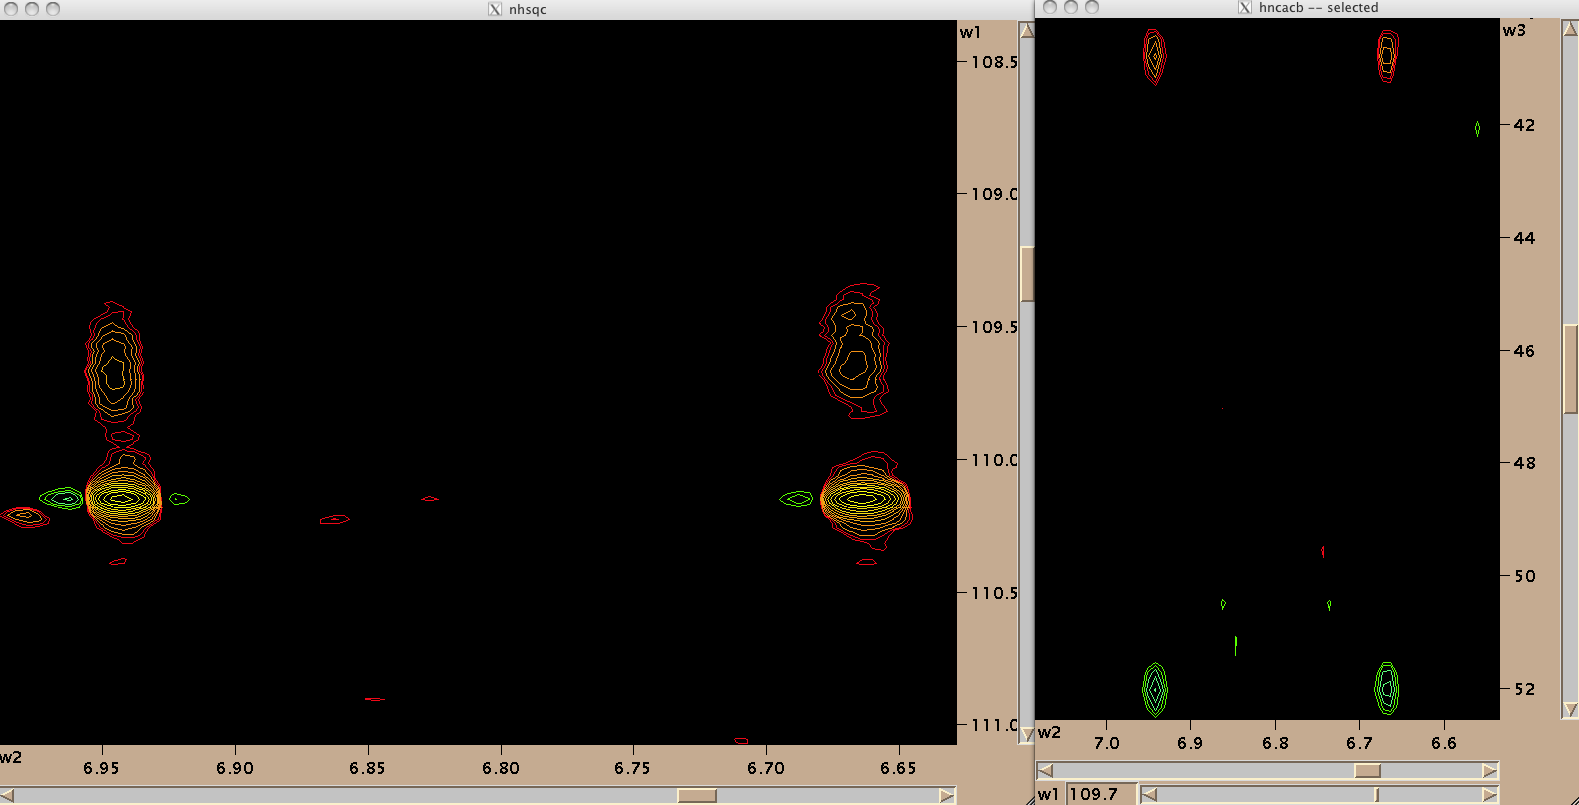
\includegraphics[scale=0.25]{figures/asn_sidechain}
  \caption{An Asparagine sidechain in the NHSQC and HNCACB spectra.}
  \label{asn_sidechain}
\end{figure}

\begin{figure}
  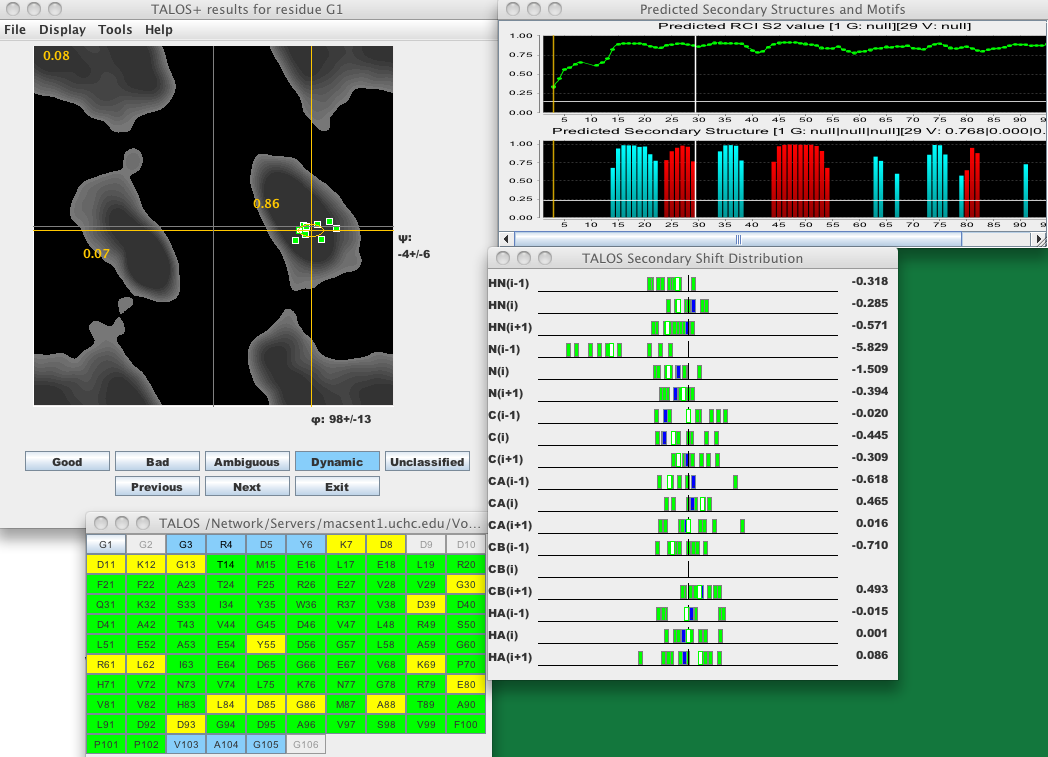
\includegraphics[scale=0.25]{figures/talos+_results}
  \caption[The secondary structure prediction according to Talos+.]
          {The torsion angles and secondary structure prediction 
           according to Talos+, along with a confidence interval.  
           These results can be shown in a Ramachandran plot.}
  \label{talos+_results}
\end{figure}

\begin{figure}
  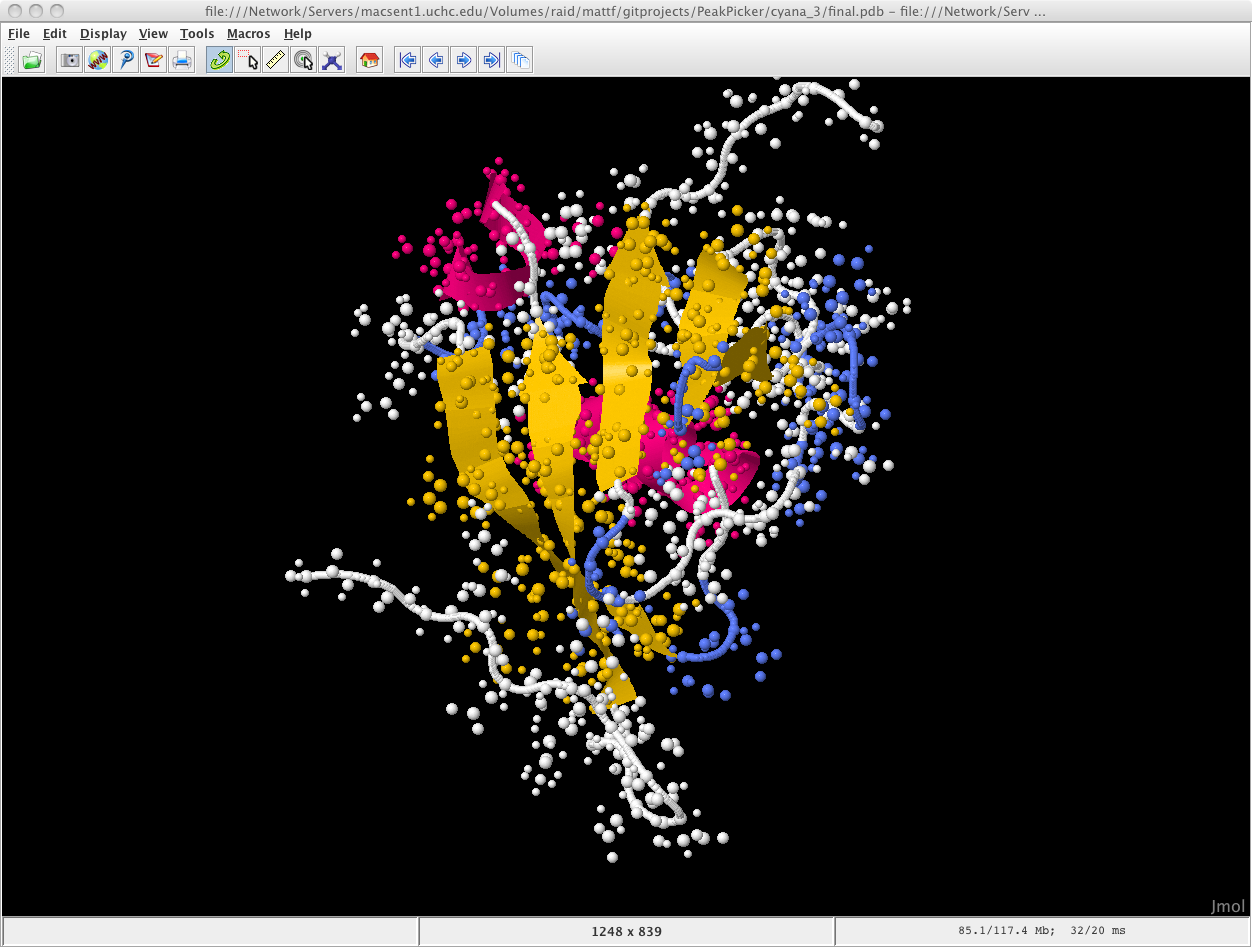
\includegraphics[scale=0.25]{figures/structure}
  \caption[The final structure as seen in jmol.]
          {The final structure as seen in jmol.
           Secondary structure is visible: beta-sheets as parallel and
           anti-parallel arrows, and alpha-helices as coiled ribbons.}
  \label{structure}
\end{figure}

\begin{figure}
  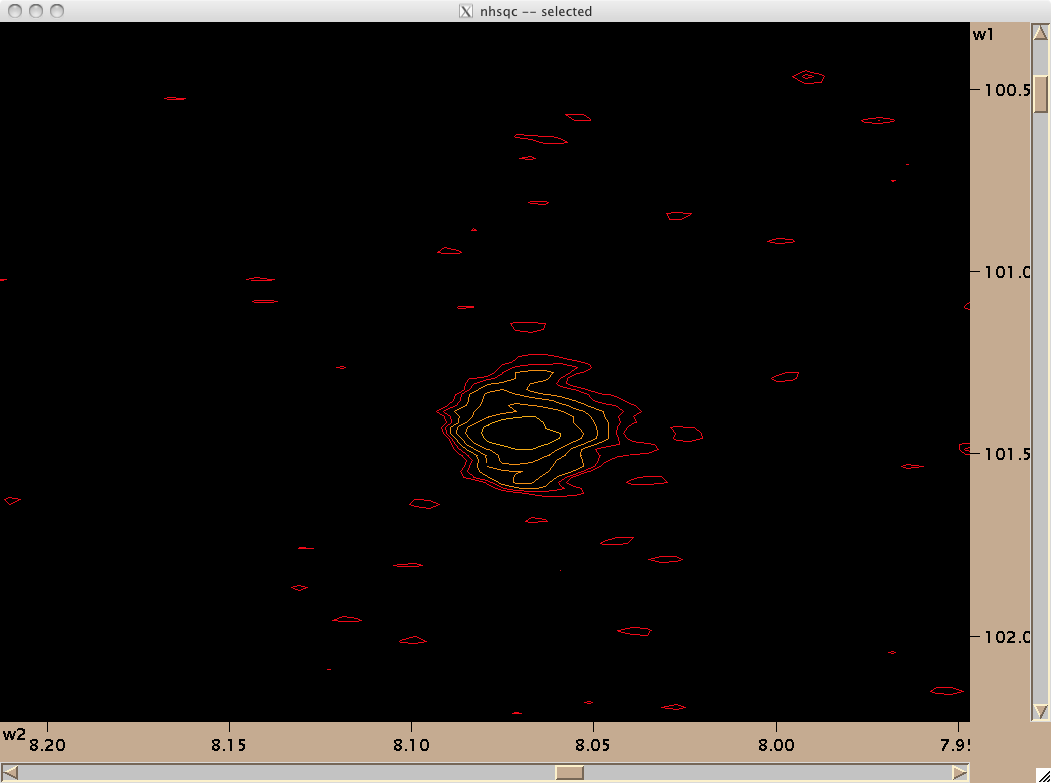
\includegraphics[scale=0.25]{figures/false_negative}
  \caption[A false negative -- a true signal missed by the automated peak picker.]
          {A false negative -- a true signal missed by the automated peak picker.
           Its intensity compared to the spectral noise level, as well as 
           peaks in additional spectra whose frequencies in multiple cross
           sections match this peak, indicate that it is a true peak.}
  \label{false_negative}
\end{figure}

\begin{figure}
  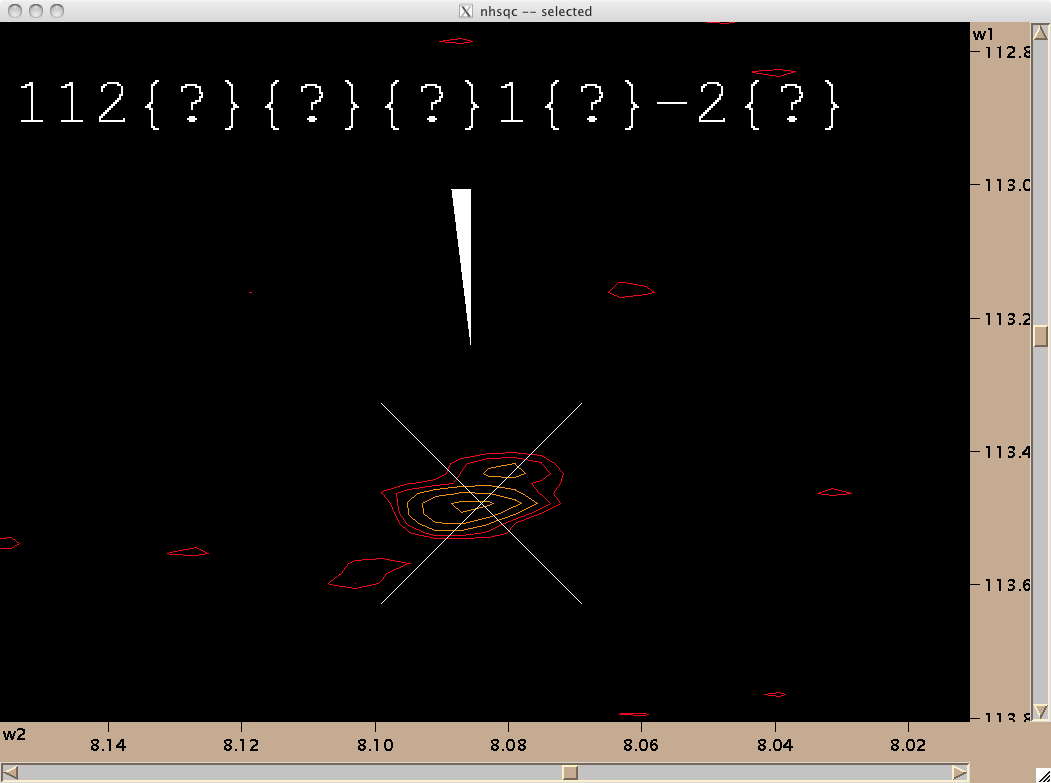
\includegraphics[scale=0.25]{figures/extraneous_gss}
  \caption{An extraneous GSS.  It was not assigned to any specific residue.}
  \label{extraneous_gss}
\end{figure}

